\documentclass[preprint,12pt]{elsarticle}
\usepackage{graphicx}
\usepackage{amsmath}
\usepackage{hyperref}
\usepackage{url}
\usepackage{tikz}
\usetikzlibrary{arrows.meta,positioning}

\journal{SoftwareX}

\begin{document}

\begin{frontmatter}

\title{KherveCAD: an open parametric modeller that language-model agents can drive}

\author[aff1]{Gwilherm Kerherve\corref{cor1}}
\ead{[email]}
\cortext[cor1]{Corresponding author}
\address[aff1]{[Affiliation]}

\begin{abstract}
KherveCAD is a desktop modeller written in Python and Qt that keeps every design as a tree of objects, and that tree compiles one-to-one into an OpenSCAD program. Because the tree and the program cannot drift apart, a part drawn with the mouse can be edited as code and a program pasted in comes back as editable objects. The application also exposes its editing operations through the Model Context Protocol (MCP). A language-model assistant connected this way does not stop at writing code: it can look at a render of what it built, measure volumes, test a part for 3D printing and check whether two parts collide, and then correct its own work. We describe the architecture, give three worked examples (a printable hinge, an ultra-high-vacuum chamber layout and a carbon nanotube), and discuss where the tool has been useful in teaching and laboratory design.
\end{abstract}

\begin{keyword}
computer-aided design \sep OpenSCAD \sep Model Context Protocol \sep large language models \sep parametric modelling \sep 3D printing
\end{keyword}

\end{frontmatter}

\section*{Code metadata}
\begin{table}[h]
\small
\begin{tabular}{|l|p{6.2cm}|p{6.2cm}|}
\hline
\textbf{Nr} & \textbf{Code metadata description} & \textbf{Value} \\ \hline
C1 & Current code version & v0.1.[N] \\ \hline
C2 & Permanent link to code/repository & \url{https://github.com/gkerherve/KherveCAD} \\ \hline
C3 & Permanent link to reproducible capsule & [Zenodo DOI] \\ \hline
C4 & Legal code licence & GPL-3.0 \\ \hline
C5 & Code versioning system used & git \\ \hline
C6 & Software code languages, tools and services used & Python 3.11+, PyQt5, OpenSCAD (optional), manifold3d, numpy \\ \hline
C7 & Compilation requirements, operating environments and dependencies & Windows 10/11, macOS (Apple silicon and Intel); see \texttt{requirements.txt} \\ \hline
C8 & Link to developer documentation/manual & Built-in user guide (F1); \texttt{docs/MCP.md} \\ \hline
C9 & Support email for questions & [email] \\ \hline
\end{tabular}
\end{table}

\section{Motivation and significance}

Scientists often need small custom parts: a sample holder, a flange adapter, a bracket for an optical bench. Commercial CAD packages handle this well but are expensive and slow to learn, so many researchers turn to OpenSCAD~\cite{openscad} instead. OpenSCAD describes a solid as a short program, which makes a design easy to version, share and tweak by changing a number. The price is that everything must be typed. Nothing can be dragged, and a beginner has to picture the shape in their head before seeing it.

Language models have changed this picture somewhat. Several groups have shown that an LLM can produce CAD from a description, either as sketch-and-extrude sequences~\cite{wu2023cadllm,khan2024text2cad} or as scripts in CadQuery and similar languages~\cite{xie2025textcadquery,guan2025cadcoder}. In practice the code often compiles but the part is wrong --- a hole on the wrong face, two pieces that overlap, a wall too thin to print --- and the model has no way of knowing. Alrashedy et al.~\cite{alrashedy2025cadcodeverify} showed that letting a vision-language model inspect renders of its output and revise the code improves results, and Sadik and Bujny~\cite{sadik2025hitl} argue that geometric metrics are needed to judge such output at all.

KherveCAD was built to close both gaps. On the human side it gives OpenSCAD a graphical editor in which shapes are drawn, moved and combined by hand, while the program stays visible and editable in a code tab (Fig.~\ref{fig:window}). On the machine side it offers the same editor to an AI assistant through the Model Context Protocol~\cite{mcp}, an open standard for connecting assistants to tools. The assistant gets the operations a person would use, plus the means to inspect the result. Our view is that this inspection step, more than code generation itself, is what makes AI-assisted design dependable enough for laboratory work.

\begin{figure}[t]
\centering
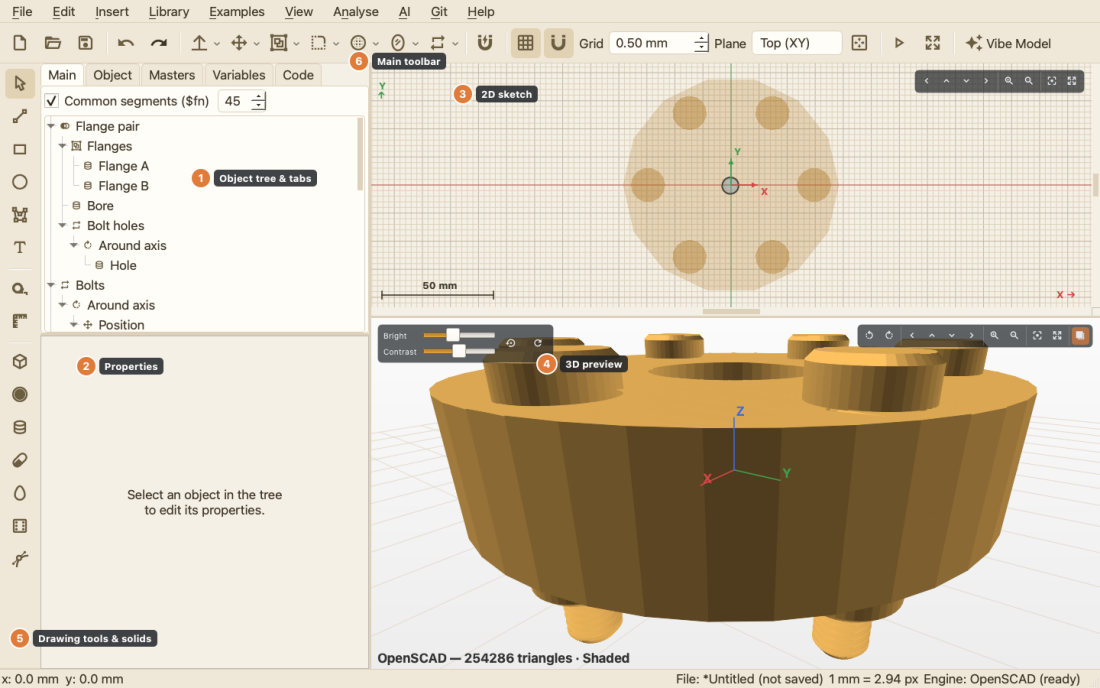
\includegraphics[width=\linewidth]{figures/fig5_window.png}
\caption{The main window: object tree (1), properties (2), 2D sketch and assembly view (3), 3D preview (4), drawing tools (5) and main toolbar (6).}
\label{fig:window}
\end{figure}

\section{Software description}

\subsection{Architecture}

The whole program rests on one rule: the object tree is the only copy of the design (Fig.~\ref{fig:arch}). Each node --- a cube, an extrusion, a translation, a boolean difference, a loop --- corresponds to exactly one OpenSCAD statement. The code shown to the user is regenerated from the tree after every change, and code typed by the user goes through a parser that rebuilds the tree. A round trip from tree to code and back is lossless, and the test suite checks it.

\begin{figure}[t]
\centering
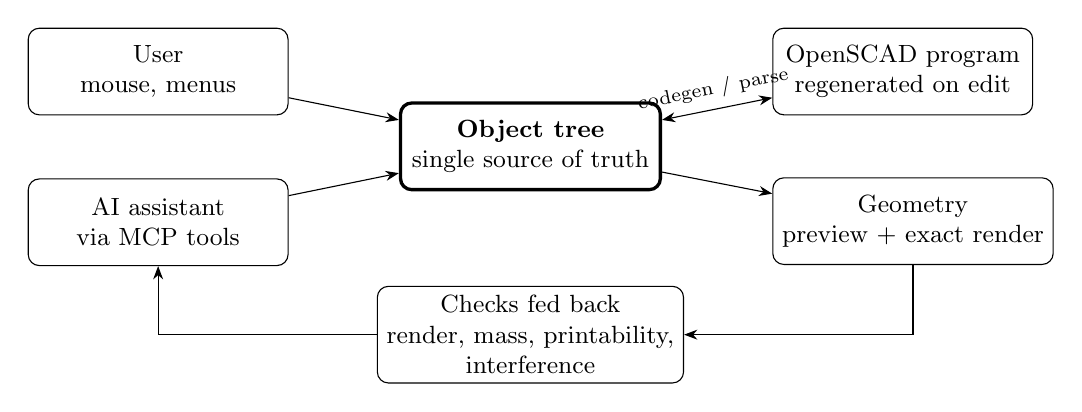
\begin{tikzpicture}[font=\small, box/.style={draw, rounded corners, align=center, minimum width=3.3cm, minimum height=1.1cm}, >=Stealth]
\node[box] (user) {User\\mouse, menus};
\node[box, below=0.8cm of user] (ai) {AI assistant\\via MCP tools};
\node[box, very thick, right=1.4cm of user, yshift=-0.95cm] (tree) {\textbf{Object tree}\\single source of truth};
\node[box, right=1.4cm of tree, yshift=0.95cm] (code) {OpenSCAD program\\regenerated on edit};
\node[box, right=1.4cm of tree, yshift=-0.95cm] (geo) {Geometry\\preview + exact render};
\node[box, below=1.2cm of tree] (chk) {Checks fed back\\render, mass, printability,\\interference};
\draw[->] (user) -- (tree);
\draw[->] (ai) -- (tree);
\draw[<->] (tree) -- node[above, sloped, font=\scriptsize]{codegen / parse} (code);
\draw[->] (tree) -- (geo);
\draw[->] (geo) |- (chk);
\draw[->] (chk) -| (ai);
\end{tikzpicture}
\caption{Architecture. The mouse and the assistant edit the same tree; the assistant also receives the results of the checks.}
\label{fig:arch}
\end{figure}

Geometry is shown in two stages. A tessellator written in Python draws an immediate preview, with boolean operations cut by the Manifold library~\cite{manifold} when it is installed. OpenSCAD then renders each part separately in the background, and the exact mesh replaces the preview as it arrives. Rendering per part rather than per document keeps each part's colour and means that moving one part re-renders nothing.

Parts are organised the way most engineering CAD does it. An \emph{Object} is a part definition that compiles to an OpenSCAD \texttt{module}, and the main tab is an assembly of placed instances. Instances can be mated face to face (flush, concentric, hinge, gear ratio), and the program still reads as plain OpenSCAD.

\subsection{The assistant interface}

The MCP server exposes 88 tools. Rather than describe them all, it helps to say what kind they are. Some edit the tree directly, such as adding a node or setting a parameter; the most used, \texttt{apply\_code}, takes an OpenSCAD program and parses it into real nodes, so the user can still drag a corner afterwards. Others only read. \texttt{render\_view} returns an image of the model from a chosen angle, so the assistant sees what it made. \texttt{check\_printability} reports open edges, overhangs and thin walls. \texttt{mass\_properties} and \texttt{check\_interference} give numbers it can compare against the brief.

The server listens only on the local machine and needs a per-session token. The user picks how much the assistant may do: read only, edit the open document, or also read and write files. Each tool call becomes a single undo step, so the person at the keyboard can reverse anything the assistant did with Ctrl+Z.

\subsection{Other functions}

Around this core sit tools that grew from our own needs. These include fillets picked on an edge, shelling, patterns, sculpting, sheet metal with flat patterns, 2D engineering drawings and STEP export through Open CASCADE~\cite{occt}. There is also a part library, which ranges from ISO fasteners and CF vacuum flanges to laboratory glassware, as well as builders for crystal structures, surfaces cut along any $(hkl)$, molecules from SMILES and peptides.

\section{Illustrative examples}

\paragraph{A print-in-place butt hinge} The hinge is three Objects: two leaves and a removable pin (Fig.~\ref{fig:hinge}). Each is placed in its own print orientation. Clearances between knuckles and around the pin are named variables, so changing the printer tolerance is a one-line edit. The shipped file is generated by a script, and a test renders it with OpenSCAD to confirm that every piece is watertight and that the leaves swing a full 180\textdegree{} without touching.

\begin{figure}[t]
\centering
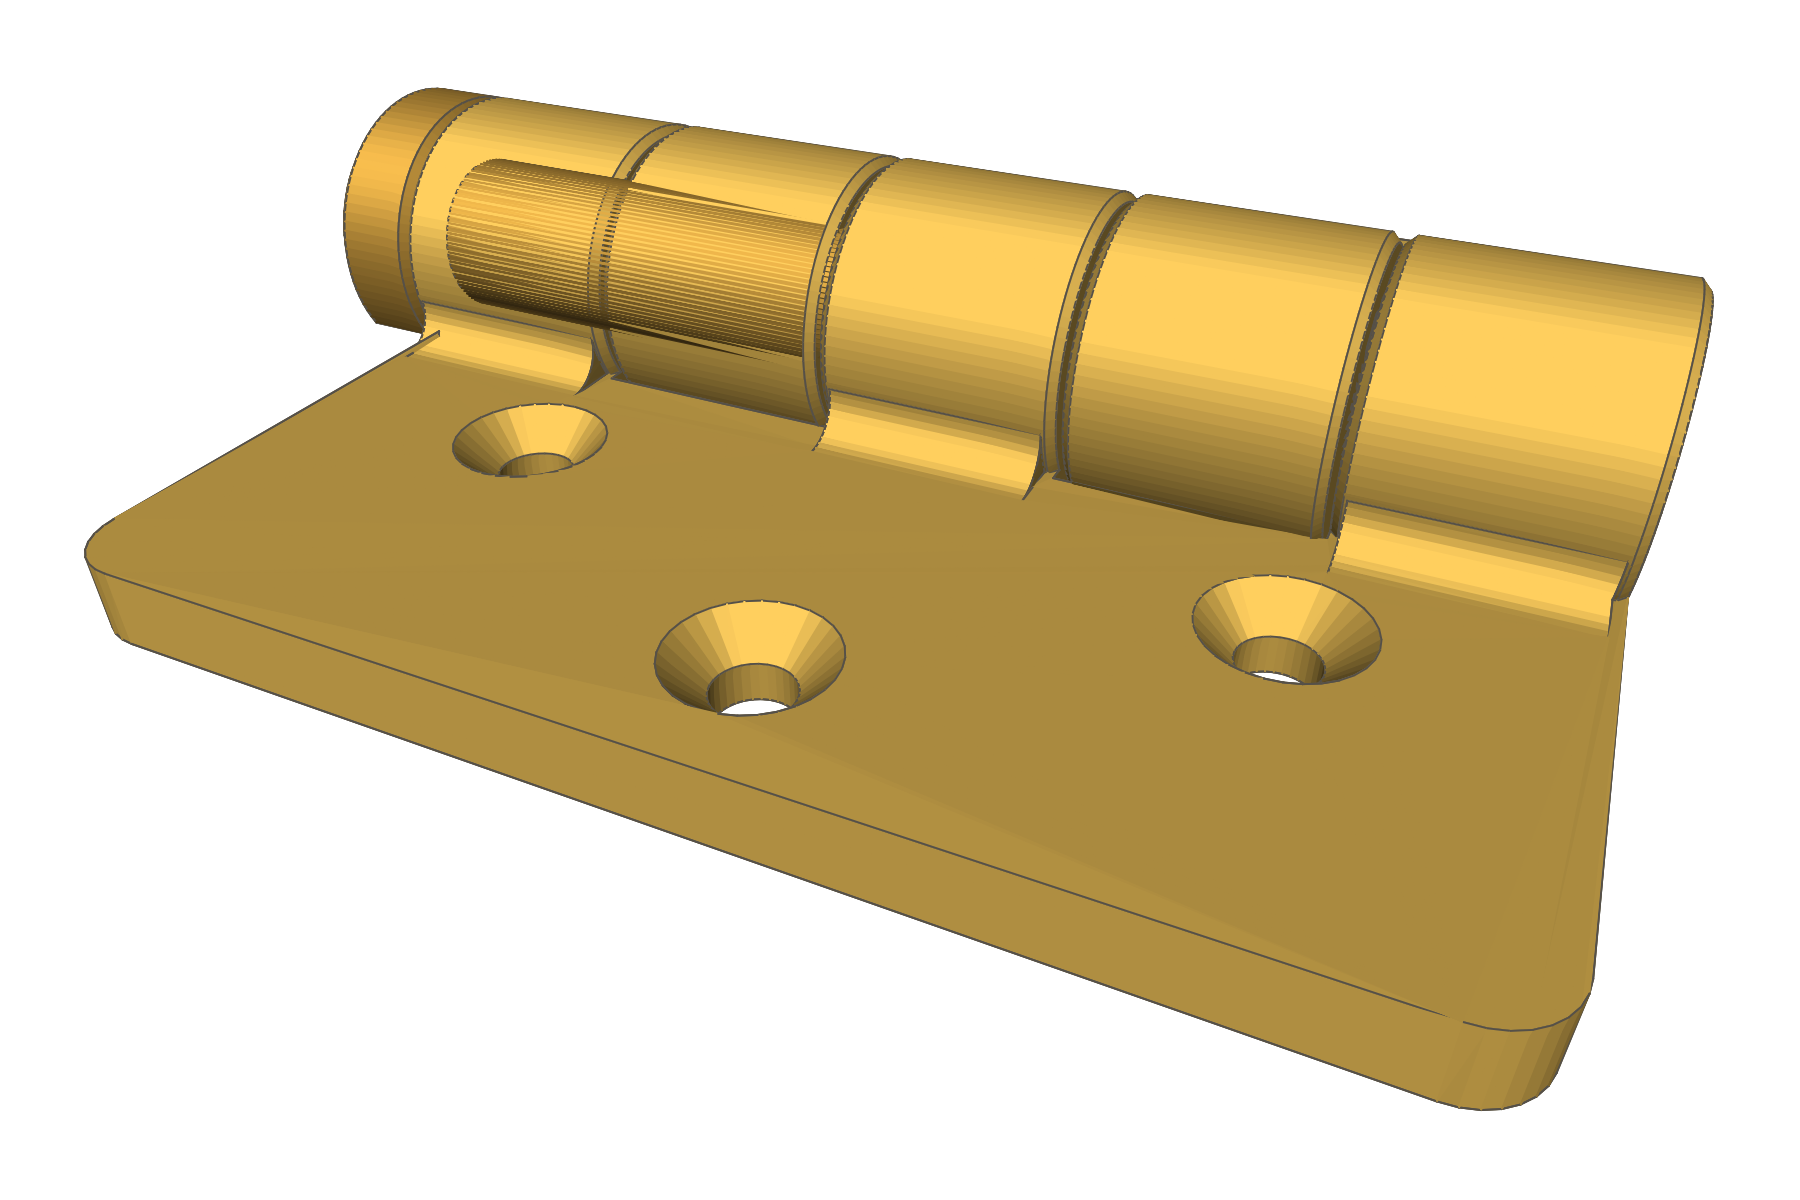
\includegraphics[width=0.8\linewidth]{figures/fig2_hinge.png}
\caption{Butt hinge with removable threaded pin, as rendered by OpenSCAD inside KherveCAD.}
\label{fig:hinge}
\end{figure}

\paragraph{An ultra-high-vacuum chamber} The Chamber Designer takes a chamber body and a list of ports, each aimed at a focal point on the axis, and fills them with flanges and instruments from the library (Fig.~\ref{fig:chamber}). It reports clashes between ports in 3D before anything is ordered. All port-mounted parts follow one convention --- sealing face at $z = 0$, vacuum side down --- so any instrument fits any port of the right flange size.

\begin{figure}[t]
\centering
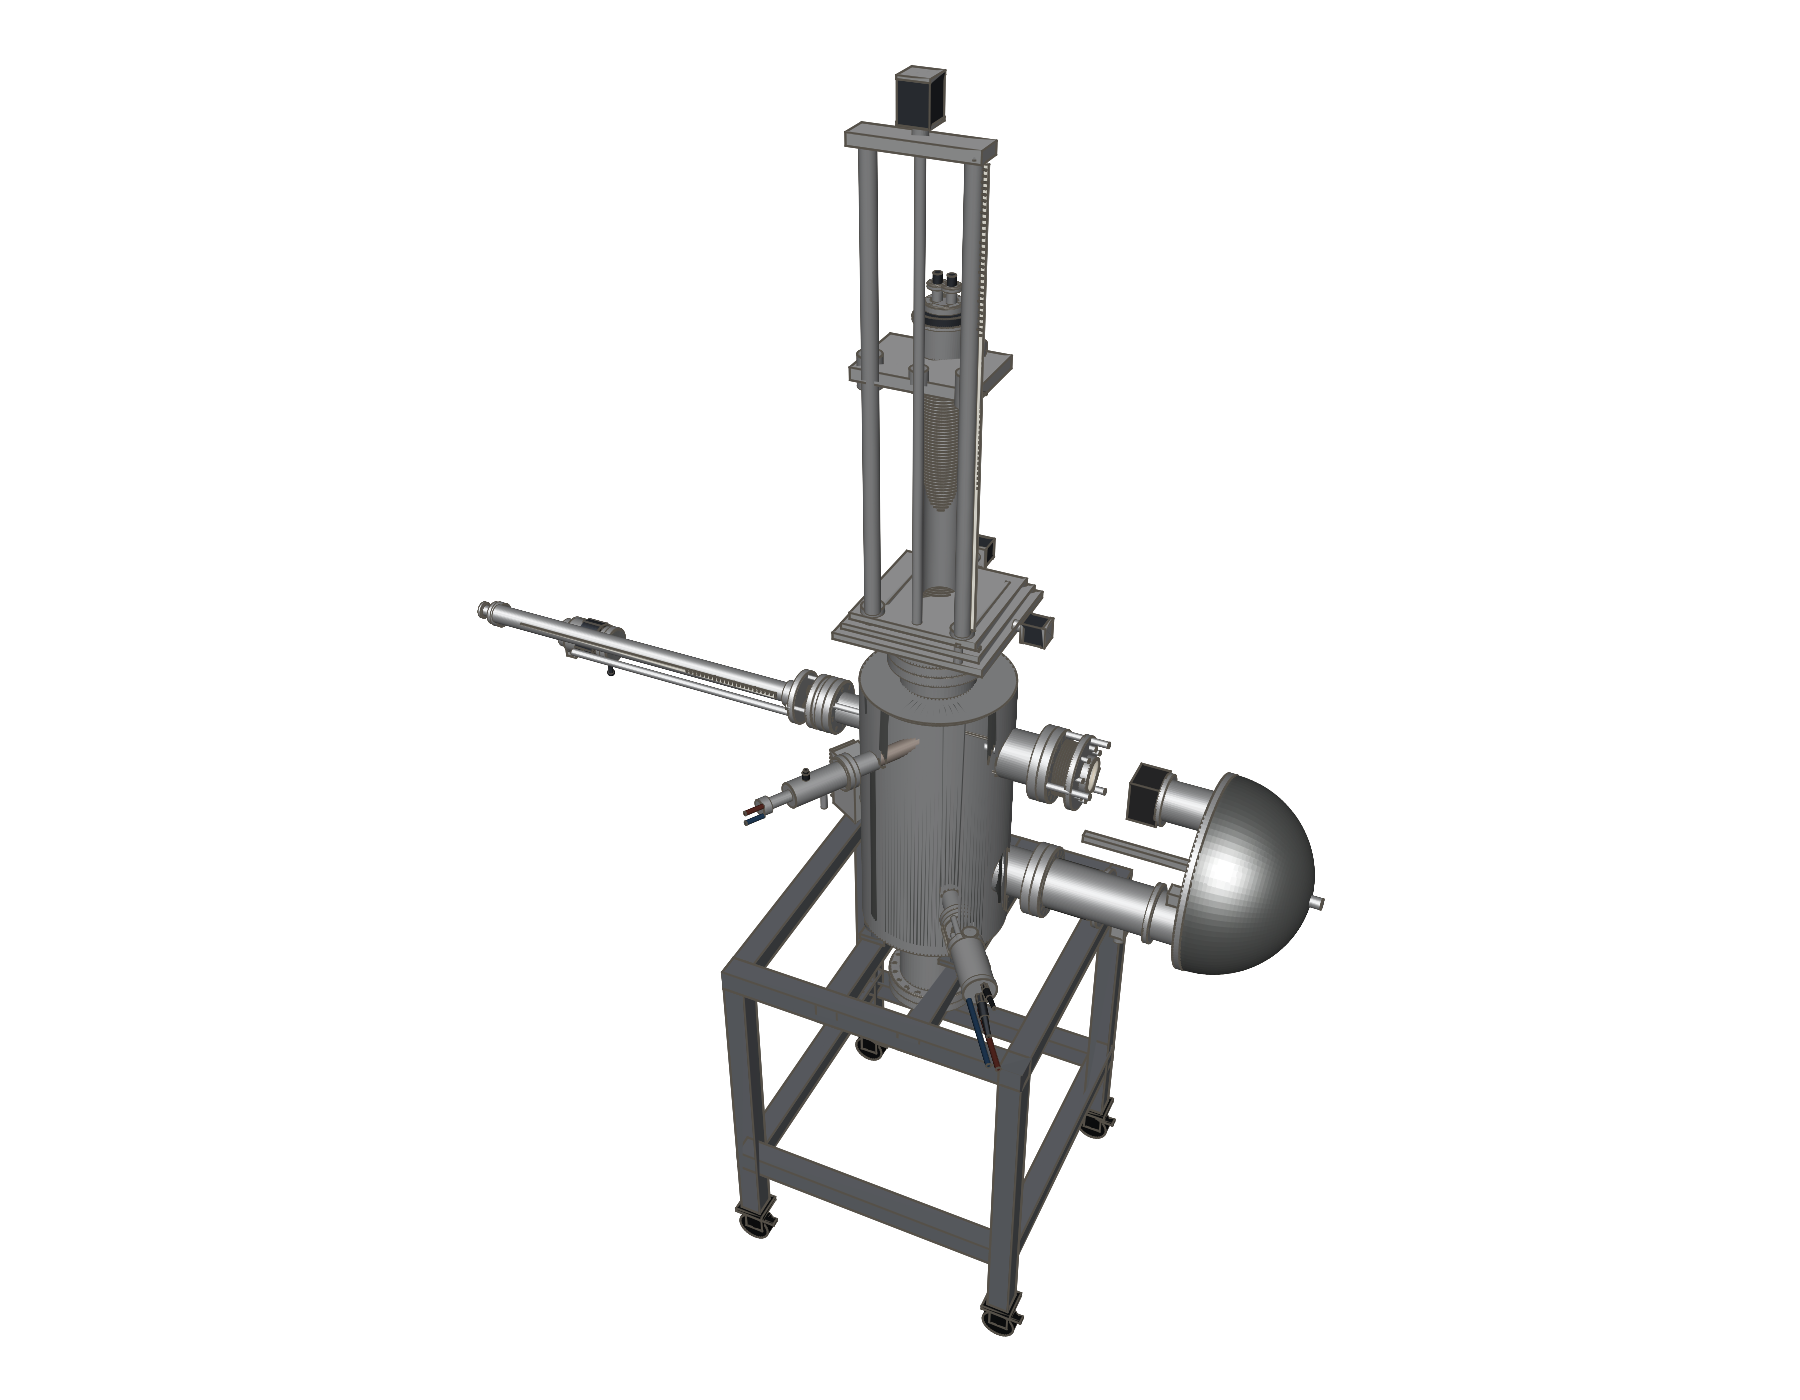
\includegraphics[width=0.75\linewidth]{figures/fig3_chamber.png}
\caption{Two-level chamber from the Chamber Designer: manipulator on top, transfer arm, hemispherical analyser and source ports, on a frame with castors.}
\label{fig:chamber}
\end{figure}

\paragraph{A carbon nanotube} Carbon nanostructures are built on their lattice rather than from a list of coordinates. An $(n, m)$ nanotube is rolled from a graphene strip along the chiral vector, so the seam closes exactly and the axis stays on $z$; graphene sheets, nanoribbons and fullerenes come from the same module. Fig.~\ref{fig:cnt} shows an $(8, 8)$ armchair tube 4\,nm long in ball-and-stick style. The document switches to nanometres on insertion, and the structure remains an editable group of atoms and bonds. The same structures are available to an assistant through \texttt{insert\_part}. [Describe here a real assistant session: the request, the tool calls and any correction it made after looking at the render.]

\begin{figure}[t]
\centering
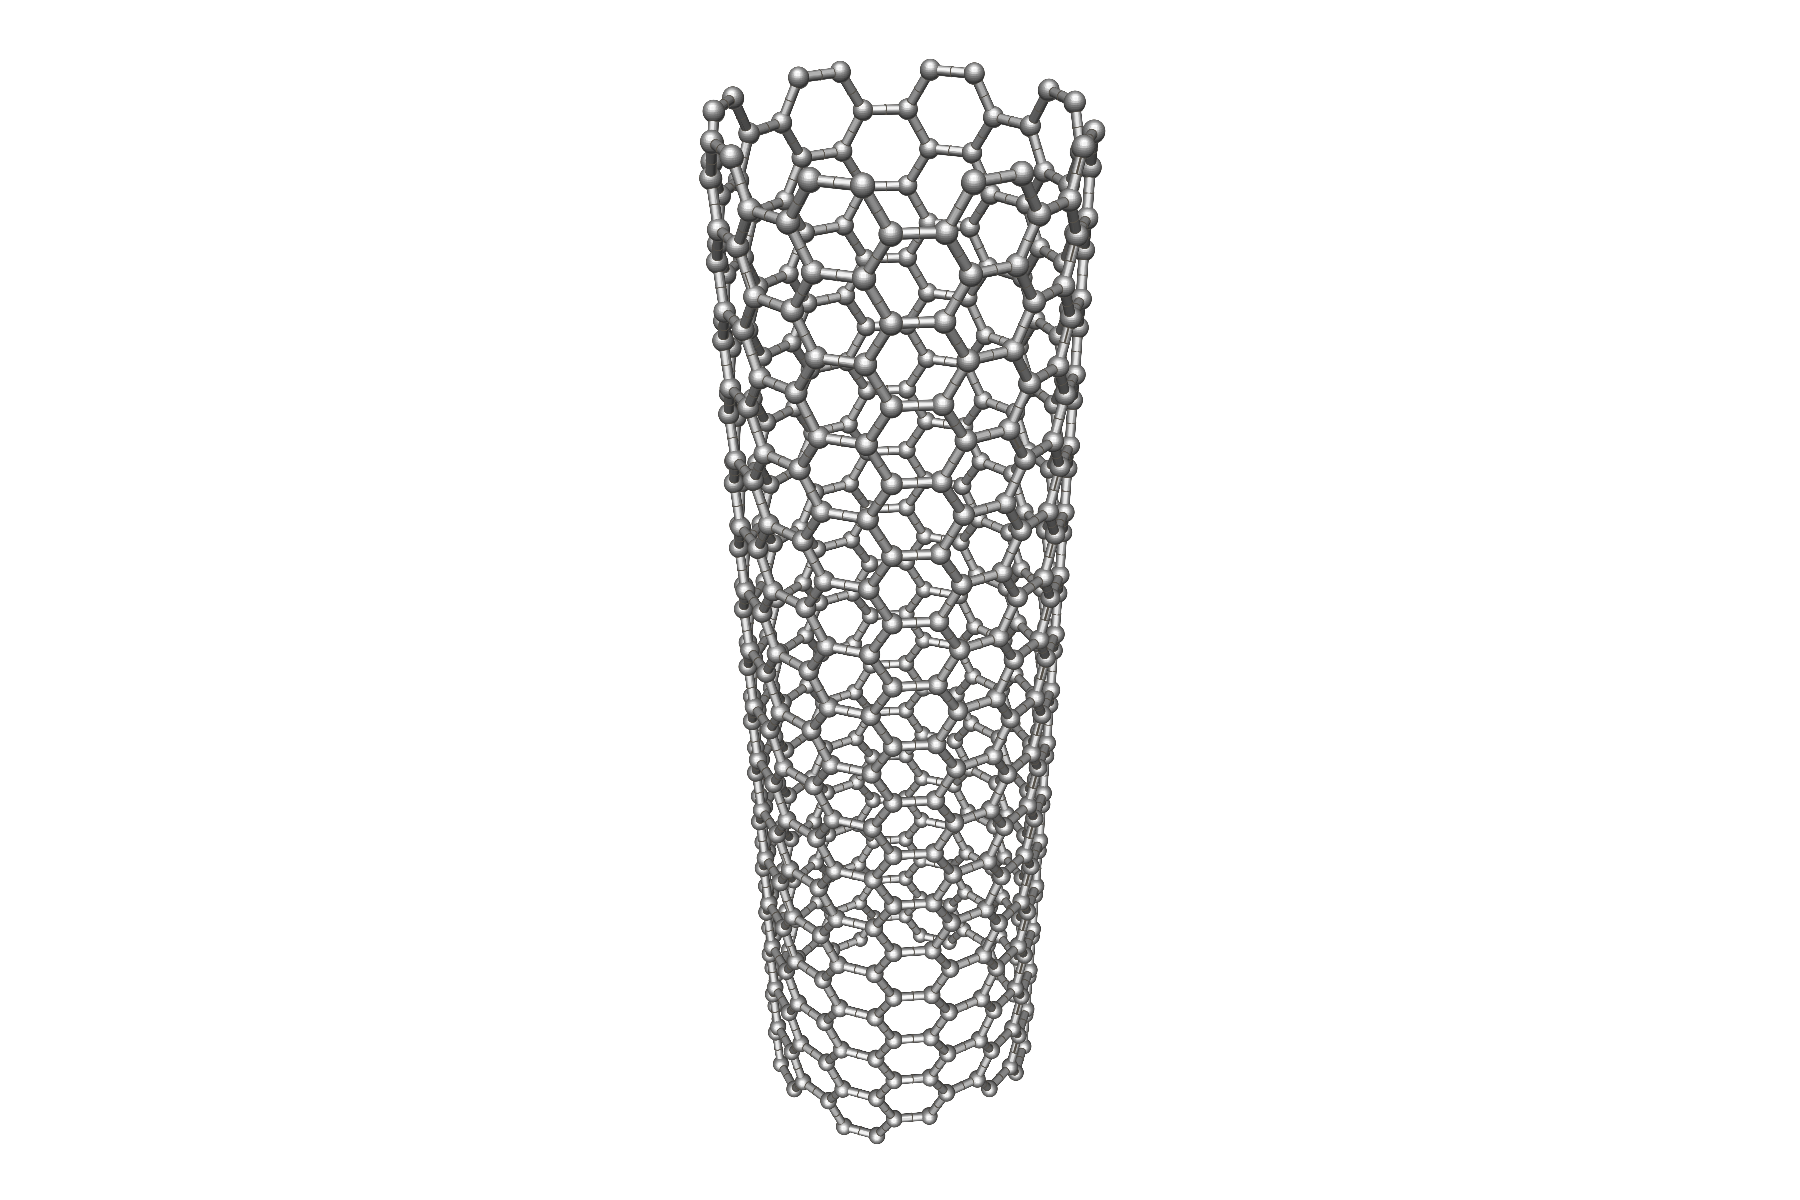
\includegraphics[width=0.75\linewidth]{figures/fig4_nanotube.png}
\caption{$(8,8)$ armchair carbon nanotube, 4\,nm long, ball-and-stick.}
\label{fig:cnt}
\end{figure}

\section{Impact}

The first use was in our own laboratory, where chambers, sample holders and adapters had been drawn in a mix of commercial CAD and hand sketches. Keeping them as short programs in one repository made them easier to revise when a port moved or a flange size changed. [Add concrete cases.]

The second use is teaching. The 21 tutorials included in the application take a student from a single cube to loops and modules, and because the code tab follows every click, students see the program grow as they draw. [Add course, number of students, feedback.]

The third, and probably the most interesting for other researchers, is as a test bed for AI-assisted design. Most published text-to-CAD work evaluates code that was generated once and then compiled~\cite{khan2024text2cad,guan2025cadcoder}. KherveCAD makes it possible to study the loop instead: an agent that builds, looks, measures and corrects, in the spirit of~\cite{alrashedy2025cadcodeverify} but with checks that go beyond the image. The same tools are available to any MCP client, so different models can be compared on identical tasks without writing a new harness for each.

The software has been publicly available since [date]. [Add downloads, stars, external users.]

\paragraph{Limitations} The built-in preview approximates some operations until OpenSCAD has rendered them. Sketches have no geometric constraint solver yet. The assistant's results also depend on the language model behind it; the tools make errors visible but do not prevent them.

\section{Conclusions}

KherveCAD puts a graphical editor on top of OpenSCAD without hiding the code, and it lets an AI assistant use that editor with the same operations a person has. The design choice that matters most is the single tree behind both. Next steps are a sketch constraint solver and a public benchmark of design tasks for comparing language models inside the tool.

\section*{Declaration of competing interest}
The author declares no competing financial interests or personal relationships that could have influenced the work reported in this paper.

\section*{Declaration of generative AI and AI-assisted technologies in the writing process}
During the preparation of this work the author used Claude (Anthropic) to help write code and draft text. After using this tool, the author reviewed and edited the content as needed and takes full responsibility for the content of the publication.

\section*{Acknowledgements}
[To fill in.]

\bibliographystyle{elsarticle-num}
\bibliography{references}

\end{document}
